\section{\label{sec:clas.ec}Electromagnetic Calorimeters (\abbr{EC})}

The final layer of the \abbr{CLAS} detector is the electromagnetic calorimeter (\abbr{EC})\cite{clas.ec}, shown in Fig.~\ref{fig:clas}. It consists of alternating layers of lead and scintillator. The overall shape is an equilateral triangle and each layer of scintillator consists of 36 strips as shown in Fig.~\ref{fig:clas.ec}. The \abbr{EC} is divided into an \emph{inner} and \emph{outer} section where the energy deposited from incident tracks is recorded separately.

\begin{figure}\begin{center}

\includegraphics[width=\figwidth]{\figures/hall-b/ec.pdf}
\caption[Electromagnetic Calorimeter Layers]{\label{fig:clas.ec}{\coloronline}Separated view of one sector of the forward electromagnetic calorimeter (\abbr{EC}) showing the three planes ($u$, $v$, $w$) of scintillator-lead pairs which make up one of the 13 \emph{logical} layers.}
\end{center}\end{figure}

The \emph{inner} layer consists of 8 \emph{logical} layers of lead and scintillator while the \emph{outer} layer consists of 5. Each \emph{logical} layer is made of three scintillator-lead layer pairs where the scintillator strips are turned 120$^\circ$ from each other, labeled $u$, $v$ and $w$. There are a total of 39 scintillator-lead layer pairs in each sector of the \abbr{EC}. The angular acceptance of the \abbr{EC} is shown in Fig.~\ref{fig:clas.ec.coverage}. Notice that it covers the entire \v{C}erenkov (Fig.~\ref{fig:clas.cc.coverage}) acceptance region.

\begin{figure}\begin{center}
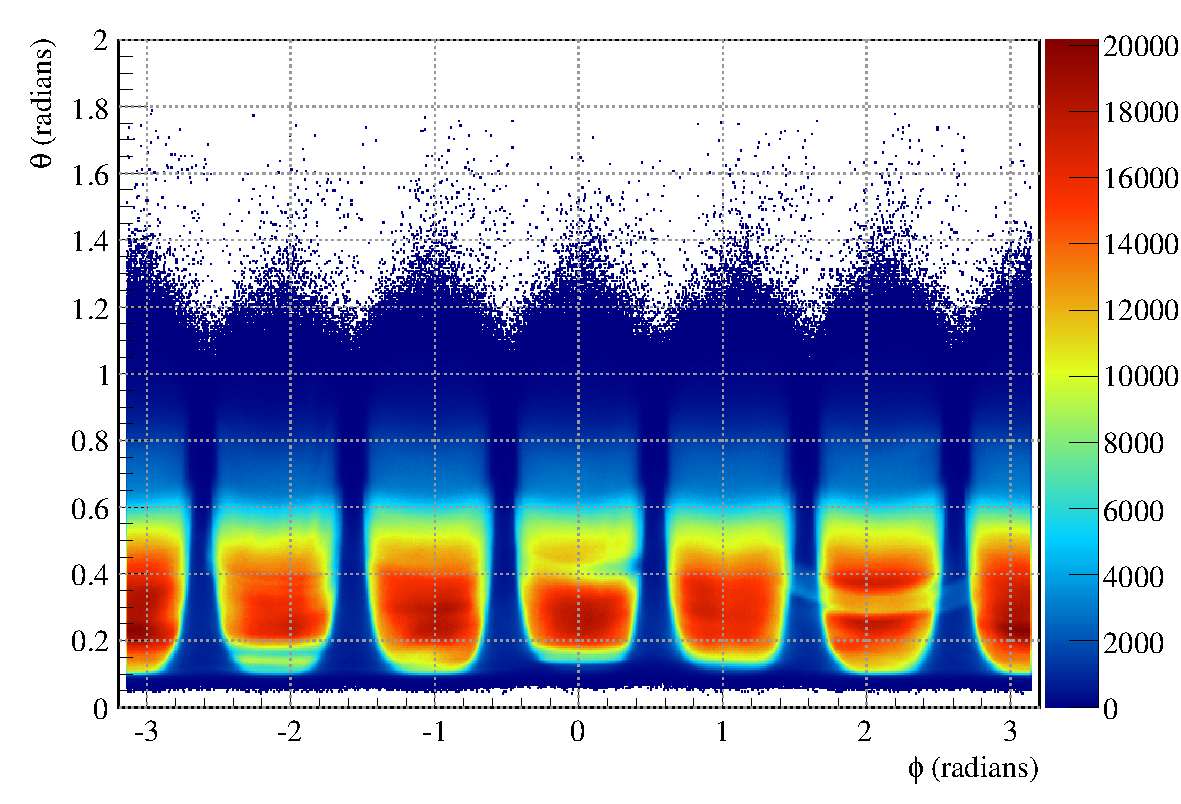
\includegraphics[width=\figwidth]{\figures/reconstruction/coverage_ec.pdf}
\caption[Electromagnetic Calorimeter Angular Coverage]{\label{fig:clas.ec.coverage}{\coloronline}Angular coverage in the lab frame of the tracks that had an associated electromagnetic calorimeter hit.}
\end{center}\end{figure}

The lead to scintillator thickness ratio (0.2) was chosen so one third of the showering particle's energy is deposited into the scintillator. Using the three layers in each \emph{logical} layer to provide pixel-like information, the transverse shower development for a given particle can be determined. The difference in energy deposit between the \emph{inner} and \emph{outer} layers provides separation of electrons from pions in the reconstructed data. For this analysis, the \abbr{EC} was used as a secondary time-of-flight measurement as well as an energy loss determination which provided additional information on particle identification. Furthermore, all final-state photons were identified in the \abbr{EC} by a signature that consisted of a hit only in the first layer of scintillators since the photons are absorbed in the leading sheet of lead.
